\chapter{Inflation, Vacuum Energy, and the de Sitter Mechanism}

Inflation is the announced subject of this lecture, but it is not the true beginning of the argument. We first go back to a simpler piece of cosmology and isolate the mechanism on which everything else will rest: a constant vacuum-energy density makes the Hubble rate constant, and a constant Hubble rate gives exponential expansion. Only after that do we return to the present accelerated universe, the cosmic horizon, the meaning of vacuum energy, and finally to the conjecture that the same de Sitter mechanism once operated in the remote past with a vastly larger effective vacuum energy. From there the lecture turns to the scalar field \(\phi\), its potential \(V(\phi)\), slow drift along a high plateau, reheating at the cliff, and the survival of just enough fluctuation to seed galaxies.

\paragraph{Credit.} These companion notes follow Leonard Susskind's Lecture 7, with supporting frame extraction curated by LazyingArt LLC and Video2Book.

\section{Vacuum Energy, de Sitter Space, and Exponential Expansion}

We begin with the flat-space Friedmann equation. The lecturer speaks of \(A(t)\); here we write the same scale factor as \(a(t)\):
\begin{equation}
\left(\frac{\dot a}{a}\right)^2=\frac{8\pi G}{3}\rho .
\end{equation}
The three basic cases discussed earlier in the course are then recalled in one stroke:
\begin{equation}
\rho_{\mathrm{matter}}\propto a^{-3},\qquad
\rho_{\mathrm{rad}}\propto a^{-4},\qquad
\rho_{\mathrm{vac}}=\rho_0=\text{constant}.
\end{equation}
The present lecture wants to isolate the third case. If the universe contains nothing but vacuum energy, then the right-hand side of the Friedmann equation is constant. We therefore define
\begin{equation}
H^2=\frac{8\pi G}{3}\rho_0,
\qquad
H=\sqrt{\frac{8\pi G}{3}\rho_0}.
\end{equation}
In this special case the Hubble parameter is truly constant:
\begin{equation}
\frac{\dot a}{a}=H.
\end{equation}
Now the differential equation is elementary but decisive:
\begin{align}
\dot a &= Ha,\\
\frac{da}{dt} &= Ha.
\end{align}
Integrating, we obtain
\begin{equation}
a(t)=a_0 e^{Ht}.
\end{equation}
So if the vacuum-energy density is constant, the distance between sufficiently separated unbound galaxies grows exponentially. This is the spacetime called de Sitter space.

The lecture also writes the metric in these expanding coordinates. Regularizing the notation into the standard line element, we have
\begin{equation}
ds^2 = dt^2 - e^{2Ht}\left(dx^2+dy^2+dz^2\right).
\end{equation}
That is the simple geometry the whole lecture keeps returning to. One should notice the logic here: inflation is not introduced as a separate miracle. It is prepared as a re-use of this exact mechanism.

A short side remark enters at this stage. If space is taken to be exactly flat, then \(H^2\) must be nonnegative, so the pure flat-space vacuum-energy solution under discussion requires nonnegative vacuum energy. The lecture mentions that negative vacuum energy can arise in non-flat cases once curvature terms are present, but that branch is not pursued here.

\section{Present Acceleration and the Cosmic Horizon}

Having rebuilt the pure de Sitter solution, the lecture turns to the present universe. The point is not that the real universe is exactly de Sitter today, but that it appears to be moving toward that behavior. In the past the scale factor followed the familiar matter-dominated law
\begin{equation}
a(t)\propto t^{2/3},
\end{equation}
whereas at late times the observed curve bends upward and approaches exponential growth.

\begin{figure}[h]
\centering
\begin{tikzpicture}[scale=0.95]
\draw (0,0) -- (6.2,0);
\draw (0,0) -- (0,4.2);
\node at (6.35,-0.15) {\(t\)};
\node at (-0.2,4.35) {\(a(t)\)};

\draw[dashed] (0.35,0.5) .. controls (1.2,1.3) and (2.3,2.0) .. (4.9,3.0);
\node at (2.2,1.15) {\(t^{2/3}\)};

\draw[line width=0.9pt] (0.35,0.5) .. controls (1.2,1.3) and (2.3,2.0) .. (3.6,2.45)
.. controls (4.3,2.7) and (5.0,3.1) .. (5.8,3.95);
\node at (4.9,2.25) {late-time};
\node at (5.0,1.95) {acceleration};
\end{tikzpicture}
\caption{Matter-dominated growth giving way to late-time accelerated expansion.}
\end{figure}

Acceleration here means exactly what one expects:
\begin{equation}
\ddot a>0.
\end{equation}
The lecture stresses that this is observational, not speculative. The observed scale factor does not yet follow a perfect exponential, but the late-time data fit smoothly onto a trend toward exponential behavior. In that sense the present universe is becoming vacuum-energy dominated.

From there the lecturer reintroduces the cosmic horizon. In proper-distance form, Hubble's law reads
\begin{equation}
v=HD.
\end{equation}
The horizon is the distance at which the recession speed reaches the speed of light. Setting \(v=c\), we get
\begin{equation}
D=\frac{c}{H},
\end{equation}
or equivalently \(HD=c\).

\begin{figure}[h]
\centering

\includegraphics[width=0.62\textwidth]{lecture_07_figure_02.png}
\caption{Hubble distance relation on the board. The secure visible relation is \(D=c/H\); the partial top line suggests the equivalent form \(HD=c\).}
\end{figure}

The board image is useful here for a structural reason. The right board isolates the horizon relation, while the left board preserves only a residue of the preceding \(\rho_0\)-to-\(H\) discussion. That is exactly the sequence of the lecture itself: first vacuum energy fixes the Hubble scale, then the Hubble scale fixes the horizon.

\subsection{Question \& Answer}

Why is \(1/H\) numerically close to the age of the universe today, and why is that not a mathematical identity?

The clean algebra is the following. If
\begin{equation}
a(t)=Ct^p,
\end{equation}
then
\begin{align}
\dot a &= Cp\, t^{p-1},\\
H=\frac{\dot a}{a} &= \frac{Cp\, t^{p-1}}{Ct^p}=\frac{p}{t}.
\end{align}
So only in the special case \(p=1\) do we get
\begin{equation}
H=\frac{1}{t}.
\end{equation}
For a matter-dominated universe, \(p=2/3\), and therefore
\begin{equation}
H=\frac{2}{3t}.
\end{equation}
Already we see that \(1/H\) need not equal the age. In exact de Sitter space the point is even sharper: \(H\) does not vary at all, while the age keeps increasing. Thus \(1/H\) is not the age of the universe. It is the characteristic e-folding time, the time over which \(a(t)\) is multiplied by \(e\). The near equality today between \(1/H\) and the age of the universe is therefore contingent, not exact.

\section{Vacuum Energy as Zero-Point Energy}

At this point the lecture takes a deliberate detour, because the audience quite reasonably asks what vacuum energy actually is. The answer given is not a complete theory of the cosmological constant. It is a lecture-level explanation of why ``empty'' space can still carry energy and why that energy need not dilute.

The model is the harmonic oscillator. Suppressing inessential numerical factors, the energy is written schematically as
\begin{equation}
E_{\mathrm{osc}}\sim p^2+x^2.
\end{equation}
Classically the ground state sits at the equilibrium point:
\begin{equation}
x=0,\qquad p=0,\qquad E=0.
\end{equation}
Quantum mechanically that configuration is forbidden by the uncertainty principle. One cannot have both \(x\) and \(p\) sharply equal to zero. Therefore the ground-state energy is positive. For the harmonic oscillator,
\begin{equation}
E_0=\frac{1}{2}\hbar\omega.
\end{equation}

Now the key lecture move is to treat fields as enormous collections of oscillators. The electromagnetic field, and indeed every quantum field, has modes; each mode behaves like an oscillator; and each oscillator contributes zero-point energy. In that schematic spirit the lecture also writes the electromagnetic energy density as
\begin{equation}
u_{\mathrm{EM}}\sim E^2+B^2.
\end{equation}
The point is not to carry out a formal canonical quantization on the spot. The point is that even when no real photons are present, the field does not settle into a truly zero-energy state. There remains zero-point energy.

\subsection{Question \& Answer}

How can ``empty'' space still carry energy?

Because in quantum theory the vacuum is not ``nothing'' in the classical sense. It is the ground state of the fields. A ground state need not have zero energy. Indeed the uncertainty principle forbids all the relevant field variables from vanishing sharply at once. So the vacuum contains no real particles in the ordinary sense, but it still carries zero-point energy.

The lecture is also careful to separate this from ordinary radiation. The three-degree background is not the vacuum energy. Radiation dilutes as the universe expands, and each photon redshifts as well. Vacuum energy, by contrast, is the residual field energy left after one has removed all removable real quanta. That is why the lecturer keeps insisting that it does not dilute.

\section{Energy, Horizons, and What Stays Fixed in de Sitter Space}

A second natural objection immediately arises. If the vacuum-energy density is constant and the universe expands, does not the total vacuum energy increase without bound? The lecture answers this cautiously. It does not produce a polished Hamiltonian treatment of general relativity. Instead it shifts the bookkeeping to the de Sitter horizon and asks what remains fixed from the viewpoint of one observer.

In exact de Sitter space the horizon size is constant:
\begin{equation}
D=\frac{c}{H}=\frac{c}{\sqrt{8\pi G\rho_0/3}}.
\end{equation}
If we estimate the vacuum energy inside the observable horizon, then
\begin{equation}
E_{\mathrm{hor}}=\frac{4\pi}{3}D^3\rho_0
=\frac{4\pi}{3}\left(\frac{c}{H}\right)^3\rho_0.
\end{equation}
Since both \(H\) and \(\rho_0\) are constant in exact de Sitter space, the vacuum energy inside that horizon volume stays constant. So from the point of view of the portion of the universe we can ever observe, the relevant amount of vacuum energy does not grow with time.

This is the part of the lecture where one has to resist the temptation to over-neaten the argument. The spoken explanation says, in effect, that general relativity mixes ordinary energy with the gravitational sector in a way that makes naive conservation-law intuition unreliable. The cleanest statement that \emph{is} secure here is the horizon statement: fixed horizon size plus fixed vacuum-energy density implies fixed observable vacuum energy in exact de Sitter space.

\subsection{Question \& Answer}

If the vacuum-energy density is constant while space expands, where does the extra energy come from?

At the level of this lecture, the safest answer is: do not think of it as a simple Newtonian bookkeeping problem over an ever-growing Euclidean box. In exact de Sitter space the cosmic horizon is fixed, so the vacuum energy within the observable region stays fixed. The lecture also says, more qualitatively, that in general relativity one is really dealing with an interplay between ordinary energy and the gravitational or expansion sector, and that the concept of ``the energy'' is subtler than in elementary mechanics. That is as far as the lecture itself wants to push the formalism here.

\section{Why Inflation Was Proposed}

Only after this reconstruction does the lecture finally return to inflation. The transition is very explicit: the same mechanism seems to have operated in the remote past, but with a much larger Hubble scale, of order
\begin{equation}
H^{-1}\sim 10^{-32}\,\mathrm{s}.
\end{equation}
Inflation is therefore not introduced as a separate law of nature. It is introduced as an earlier de Sitter-like epoch with a much larger effective vacuum energy.

What problem was that idea meant to solve? The lecture answers: flatness and homogeneity. On large scales the universe appears spatially flat and remarkably smooth. More sharply still, the surface of last scattering was already smooth. So whatever smoothed the universe cannot be a late-time process acting only between recombination and now.

The lecturer's language is visual. Suppose the early universe began like a shriveled raisin or a wrinkled balloon, with texture and inhomogeneity. Where did the wrinkles go? If one takes a deflated balloon and inflates it enough, the wrinkles become imperceptible on any local patch. That is the inflationary thought: there was a prehistory before the observable hot universe, and during that prehistory space expanded exponentially by an enormous factor.

This also answers a different concern. One does not need to assume a carefully prepared equilibrium state before inflation. Inflation erases memory of the initial conditions. Any initial blotch is stretched to scales far beyond the observable universe. The lecture likes this feature and distrusts it at the same time: inflation explains why we do not need to know the initial conditions, but precisely for that reason it hides much of the detailed prehistory.

\section{Scalar Field \(\phi\) and the Potential \(V(\phi)\)}

The next turn in the lecture is from geometry to field theory. If the remote past really behaved like de Sitter space with a much larger effective vacuum energy, what was the origin of that energy? The answer offered is a hypothetical scalar field \(\phi\).

Unlike the electromagnetic field, a scalar field has no direction at each point of space. It is just a number:
\begin{equation}
\phi=\phi(x,y,z,t).
\end{equation}
The lecture emphasizes that this field is not identified with any observed particle or known field. It is introduced because the mathematics allows such an object and because inflation seems to ask for something like it.

What matters most is its potential-energy density \(V(\phi)\). This is energy stored not in the time dependence of the field but in the field value itself. Different values of \(\phi\) can correspond to different potential energies.

\begin{figure}[h]
\centering

\includegraphics[width=0.68\textwidth]{lecture_07_figure_03.png}
\caption{The first scalar-potential sketch used in the lecture. The board notation \(V(\phi)\) is visible, and the curve makes the essential point that different values of \(\phi\) correspond to different potential energies.}
\end{figure}

If \(\phi\) is approximately constant in space and time over the region under discussion, then \(V(\phi)\) behaves exactly like a vacuum-energy density:
\begin{equation}
\rho_{\mathrm{eff}}=V(\phi).
\end{equation}
In that case the Friedmann equation becomes
\begin{equation}
H(\phi)=\sqrt{\frac{8\pi G}{3}V(\phi)}.
\end{equation}
So the rule is simple: wherever the earlier vacuum-energy discussion used \(\rho_0\), we may now, for an approximately constant scalar field, replace \(\rho_0\) by \(V(\phi)\).

\begin{figure}[h]
\centering
\begin{tikzpicture}[scale=0.95]
\draw (0,0) -- (6.2,0);
\draw (0,0) -- (0,4.2);
\node at (6.35,-0.15) {\(\phi\)};
\node at (-0.15,4.35) {\(V\)};

\draw[line width=0.9pt]
(0.35,3.55) .. controls (1.15,1.85) and (1.55,1.35) .. (2.15,1.55)
.. controls (2.8,1.8) and (3.25,3.45) .. (4.15,3.25)
.. controls (4.85,3.05) and (5.25,1.45) .. (5.8,1.0);
\end{tikzpicture}
\caption{A clean redraw of the lecture's generic \(V(\phi)\) sketch. At this stage the point is only that the potential energy depends on field value.}
\end{figure}

The lecturer then adds one more ingredient. If \(\phi\) varies from place to place, then different regions expand with different local time constants. But exponential stretching itself tends to homogenize the field on any visible patch. That is why inflation can begin with variation and still leave each observable region looking nearly constant.

\subsection{Question \& Answer}

What are the axes of the \(V(\phi)\) graph, and in what sense can \(\phi\) behave like a time parameter without being time itself?

The horizontal axis is the field value \(\phi\), and the vertical axis is the potential-energy density \(V\). So the graph is not a plot of energy versus time. It is a plot of energy versus field value.

Nevertheless, once the field rolls monotonically down the potential, the sequence of values \(\phi(t)\) can be used as a clock along that trajectory. In that limited sense \(\phi\) acts like a time parameter: later times correspond to later points along the curve. But \(\phi\) is not itself time. It is a field value whose evolution happens to be monotonic during the relevant stage of the cosmological history.

\section{Reheating, E-foldings, and Primordial Fluctuations}

The lecture now specializes to the observationally motivated shape of the potential: a high plateau, almost flat but not exactly flat; a sharp cliff; and a lower minimum which does not quite reach zero. This is the picture used to tell the inflationary story.

\begin{figure}[h]
\centering

\includegraphics[width=0.68\textwidth]{lecture_07_figure_04.png}
\caption{The inflationary potential as drawn late in the lecture: a high plateau, a sharp drop, and a lower minimum.}
\end{figure}

\begin{figure}[h]
\centering
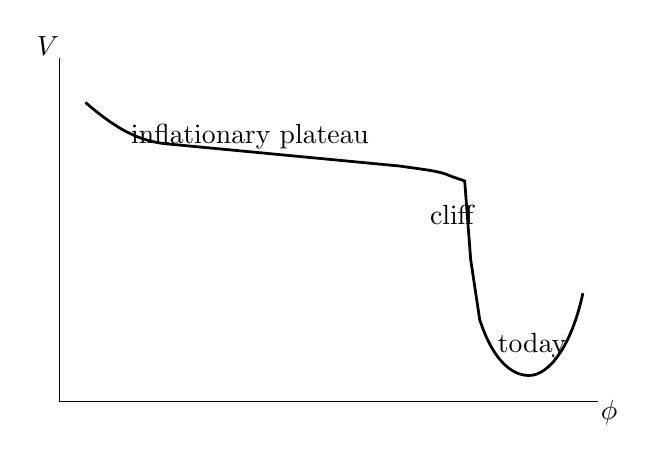
\begin{tikzpicture}[scale=0.95]
\draw (0,0) -- (7.2,0);
\draw (0,0) -- (0,4.6);
\node at (7.35,-0.15) {\(\phi\)};
\node at (-0.15,4.75) {\(V\)};

\draw[line width=1pt]
(0.35,4.0) .. controls (0.7,3.7) and (1.0,3.5) .. (1.4,3.45)
-- (4.55,3.15)
.. controls (4.9,3.1) and (5.1,3.08) .. (5.22,3.02)
-- (5.42,2.95)
-- (5.5,1.9)
-- (5.62,1.1)
.. controls (5.78,0.6) and (6.02,0.35) .. (6.28,0.35)
.. controls (6.55,0.35) and (6.85,0.75) .. (7.0,1.45);

\node at (2.55,3.55) {inflationary plateau};
\node at (5.25,2.5) {cliff};
\node at (6.32,0.75) {today};
\end{tikzpicture}
\caption{A schematic redraw of the high-plateau, cliff, and minimum structure emphasized in the lecture.}
\end{figure}

The story is then qualitative but mathematically guided. High on the plateau the potential changes very little as \(\phi\) moves, so \(V(\phi)\) is almost constant and the universe inflates almost exponentially. The field is not exactly frozen. It drifts slowly because the plateau has a small slope, and the motion is slowed by a cosmological viscosity associated with expansion. The lecture avoids writing the full field equation, but the logic is unmistakable: small slope plus large friction implies slow drift.

During this stage the scale factor grows by many e-foldings:
\begin{equation}
N=\ln\frac{a_f}{a_i}.
\end{equation}
The lecture states that one needs at least roughly \(50\) e-foldings, with \(60\) often quoted:
\begin{equation}
N\gtrsim 50,
\qquad
N\sim 60 \text{ as a common benchmark.}
\end{equation}
Each e-fold corresponds to multiplication of the scale factor by \(e\), and the corresponding timescale during inflation is quoted as roughly \(10^{-32}\,\mathrm{s}\).

When the field reaches the edge of the cliff, the potential energy changes rapidly. That energy is converted first into kinetic energy of the field and then into heat, radiation, and particles. This is the lecture's reheating transition. The universe is not hot up on the plateau; any pre-existing heat would have been diluted away by the enormous expansion. It becomes hot only after the fall.

At this point the lecture deliberately blurs and then re-sharpens the phrase ``Big Bang.'' One may, if one likes, identify reheating with the Big Bang in a loose prehistory sense. But the surface of last scattering is much later. The universe must first cool enough to become transparent. Thus what we actually observe lies far down at the bottom of the potential, not up on the inflationary plateau.

\subsection{Question \& Answer}

Why must the plateau not be perfectly flat, and how do the remaining fluctuations become structure?

If the plateau were exactly flat, there would be no classical drift produced by the slope of the potential. The lecture therefore insists that the top is not perfectly flat. It must have some tilt. At the same time it must be flat enough that \(V(\phi)\) changes only slowly and inflation lasts long enough.

But that is not the end of it. Even after enormous inflation, quantum mechanics prevents the field from becoming perfectly homogeneous. The lecture's central picture is a contour map: vertical direction ordinary space, horizontal direction field value \(\phi\), and nearly horizontal contours drifting slowly toward the cliff.

\begin{figure}[h]
\centering
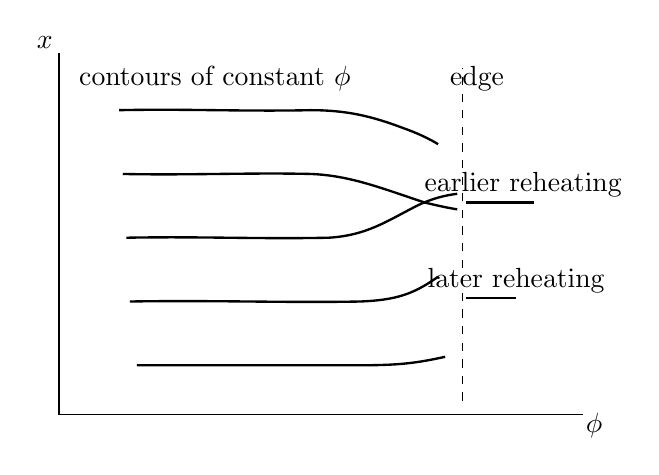
\begin{tikzpicture}[scale=0.9]
\draw (0,0) -- (7.4,0);
\draw (0,0) -- (0,5.1);
\node at (7.55,-0.15) {\(\phi\)};
\node at (-0.2,5.25) {\(x\)};

\draw[dashed] (5.7,0.2) -- (5.7,4.9);
\node at (5.9,4.75) {edge};

\draw[line width=0.85pt] (1.1,0.7) .. controls (2.2,0.7) and (3.1,0.7) .. (4.2,0.7)
.. controls (4.75,0.7) and (5.0,0.72) .. (5.45,0.82);

\draw[line width=0.85pt] (1.0,1.6) .. controls (2.2,1.62) and (3.2,1.58) .. (4.25,1.6)
.. controls (4.75,1.62) and (5.0,1.7) .. (5.35,1.95);

\draw[line width=0.85pt] (0.95,2.5) .. controls (2.0,2.52) and (2.8,2.48) .. (3.8,2.5)
.. controls (4.35,2.53) and (4.65,2.75) .. (5.05,2.95)
.. controls (5.25,3.05) and (5.45,3.1) .. (5.62,3.12);

\draw[line width=0.85pt] (0.9,3.4) .. controls (1.8,3.38) and (2.7,3.42) .. (3.55,3.4)
.. controls (4.1,3.38) and (4.55,3.2) .. (5.15,3.0)
.. controls (5.35,2.95) and (5.5,2.92) .. (5.62,2.9);

\draw[line width=0.85pt] (0.85,4.3) .. controls (1.8,4.32) and (2.6,4.28) .. (3.55,4.3)
.. controls (4.05,4.3) and (4.4,4.22) .. (4.85,4.05)
.. controls (5.05,3.98) and (5.22,3.9) .. (5.35,3.82);

\draw[line width=1pt] (5.75,3.0) -- (6.7,3.0);
\draw[line width=1pt] (5.75,1.65) -- (6.45,1.65);

\node at (2.2,4.75) {contours of constant \(\phi\)};
\node at (6.55,3.25) {earlier reheating};
\node at (6.45,1.9) {later reheating};
\end{tikzpicture}
\caption{A transcript-driven contour sketch: the field is almost homogeneous, but small quantum bumps make different regions reach the cliff at different times.}
\end{figure}

If the field were perfectly homogeneous, every region would fall off the cliff at the same moment. With quantum fluctuations, some regions fall earlier and some later. The earlier-falling region reheats first and then has more time to expand and cool. The later-falling region remains hotter and denser. Therefore the post-reheating energy density is not exactly uniform.

The lecture describes the final result by the observed amplitude
\begin{equation}
\frac{\delta\rho}{\rho}\sim 10^{-5}.
\end{equation}
These are primordial density fluctuations, not dark energy. They are small, but they are enough. After reheating, gravity amplifies over-dense regions and under-dense regions in opposite directions. The over-dense regions attract more matter, the under-dense regions are depleted, and in time the tiny initial variation becomes the seed of galaxies.

This is why the lecture treats inflation as a two-sided phenomenon. It wipes away initial irregularity and produces large-scale smoothness, but it cannot smooth the universe completely because quantum mechanics leaves a residual pattern behind. That pattern is then imprinted on the microwave background and later processed by gravity into the visible large-scale structure of the universe. The lecture ends by pointing forward: acoustic waves in that primordial plasma provide the geometric measuring rod used to determine the spatial curvature of the universe.

\section{Summary}

The lecture's logic is tighter than the word ``inflation'' by itself suggests. First one isolates pure vacuum-energy cosmology and sees that constant \(\rho_0\) gives constant \(H\), exponential growth, and de Sitter space. Then one notices that the present universe is moving toward that behavior, with a horizon scale \(D=c/H\). Student questions force the lecture to explain vacuum energy as zero-point energy and to handle horizon bookkeeping carefully. Only then does the main conjecture appear: the same de Sitter mechanism acted in the remote past with a much larger effective vacuum energy.

To model that early epoch, the lecture introduces a scalar field \(\phi\) and a potential \(V(\phi)\). A high, nearly flat plateau gives slow drift and inflation; a sharp fall gives reheating; a lower nonzero minimum leaves the tiny late-time vacuum energy we infer today. Inflation smooths the universe dramatically, but quantum fluctuations prevent exact uniformity. Different regions reheat at slightly different times, producing density contrasts of order \(10^{-5}\). Those tiny contrasts are then amplified by gravity and become the seeds of galaxies. That is the payoff of the chapter: the same mechanism that smooths the universe also leaves behind the roughness from which structure grows.